\documentclass[11pt,aspectratio=169]{beamer}
\usepackage[utf8]{inputenc}
\usepackage[T1]{fontenc}
\usepackage[main=french,provide=*]{babel}
\usepackage{graphicx}
\usepackage{booktabs}
\usepackage{amsmath}

% ---------- Thème maison (bleu Dauphine), sans dépendance externe ----------
\usetheme{default}
\useinnertheme{rounded}
\setbeamertemplate{navigation symbols}{}
\definecolor{dauphblue}{RGB}{30,70,120}
\definecolor{dauphlight}{RGB}{225,232,240}
\definecolor{accent}{RGB}{200,70,40}
\setbeamercolor{structure}{fg=dauphblue}
\setbeamercolor{frametitle}{fg=white,bg=dauphblue}
\setbeamercolor{title}{fg=dauphblue}
\setbeamercolor{alerted text}{fg=accent}
\setbeamerfont{frametitle}{series=\bfseries}
\setbeamertemplate{frametitle}{\vspace{2pt}\insertframetitle\vspace{2pt}}
\setbeamertemplate{itemize item}{\color{dauphblue}\textbullet}
\setbeamertemplate{itemize subitem}{\color{dauphblue}--}

% Intervenant courant (change à chaque bloc) -> affiché en bas
\newcommand{\speaker}{}
\setbeamertemplate{footline}{%
  \hbox{\begin{beamercolorbox}[wd=\paperwidth,ht=2.6ex,dp=1.2ex,leftskip=1em,rightskip=1em]{}%
  \color{dauphblue}\footnotesize Climateflation \& Banque Centrale
  \hfill \textbf{\speaker} \hfill \insertframenumber/\inserttotalframenumber
  \end{beamercolorbox}}}

\title{\textbf{Climat : la Banque Centrale a-t-elle un rôle à jouer ?}}
\subtitle{Une analyse de la \emph{climateflation} : SVAR, Local Projections \& allocation d'actifs}
\author{Yves-Marie Saliou\quad\textperiodcentered\quad Milos Gajic \quad\textperiodcentered\quad Marc Jehannin}
\institute{Université Paris-Dauphine -- PSL \\ Master Ingénierie Économique \& Financière}
\date{Soutenance du 13 juin}

\begin{document}

{\setbeamertemplate{footline}{}
\begin{frame}\titlepage\end{frame}}

% Plan
\begin{frame}{Plan \& répartition (\textasciitilde 5 min chacun)}
\begin{columns}[T]
\begin{column}{0.5\textwidth}
\textbf{\color{dauphblue}Partie 1 — Cadre \& méthode}
\begin{itemize}\small
\item Problématique \& cadre de Schnabel
\item Données \& choc climatique
\item Stratégie économétrique
\end{itemize}
\vspace{0.4em}
\textbf{\color{dauphblue}Partie 2 — Résultats}
\begin{itemize}\small
\item Effet agrégé (SVAR)
\item Climateflation vs fossilflation
\item Intensification \& asymétrie
\end{itemize}
\end{column}
\begin{column}{0.5\textwidth}
\textbf{\color{dauphblue}Partie 3 — Marchés \& réponse}
\begin{itemize}\small
\item Allocation d'actifs
\item Robustesse
\item La banque centrale a-t-elle un rôle ?
\item Conclusion
\end{itemize}
\end{column}
\end{columns}
\vfill
\centering\small\emph{un choc climatique se comporte comme un choc d'offre $\Rightarrow$ il crée un dilemme pour la banque centrale.}
\end{frame}

% =====================================================================
% =====================================================================
\begin{frame}[plain]
\begin{center}
{\color{dauphblue}\Large\textbf{Partie 1}}\\[0.4em]
{\large Contexte, données et stratégie économétrique}
\end{center}
\end{frame}

\begin{frame}{La question et pourquoi elle compte}
\begin{itemize}
\item Mandat premier d'une banque centrale : la \alert{stabilité des prix}.
\item Un aléa climatique agit comme un \alert{choc d'offre} : il \emph{pousse les prix à la hausse} \emph{et} \emph{pèse sur l'activité}.
\item $\Rightarrow$ Dilemme : resserrer pour l'inflation aggrave la récession.
\end{itemize}
\vfill
\textbf{\color{dauphblue}Notre angle : la \emph{climateflation}}
\begin{itemize}
\item On teste empiriquement si ce choc est \emph{gros, persistant, croissant}.
\item Trois dimensions imposées par le sujet : \alert{croissance}, \alert{inflation}, \alert{allocation d'actifs}.
\end{itemize}
\end{frame}

\begin{frame}{Cadre : les trois canaux de Schnabel (BCE, 2022)}
\begin{columns}[T]
\begin{column}{0.56\textwidth}
\begin{itemize}
\item \alert{Climateflation} : l'aléa physique désorganise l'offre (agriculture, énergie).
\item \alert{Fossilflation} : coût de la dépendance aux fossiles.
\item \alert{Greenflation} : tensions de la transition (métaux, capital).
\end{itemize}
\vspace{0.5em}
On garde la \textbf{climateflation} comme objet, la \textbf{fossilflation} comme étalon de comparaison.
\end{column}
\begin{column}{0.44\textwidth}
\small\textbf{\color{dauphblue}4 hypothèses testables}
\begin{itemize}\small
\item[H1] effet agrégé \emph{faible}
\item[H2] dominé par le \emph{fossile}
\item[H3] il \emph{s'intensifie}
\item[H4] il est \emph{asymétrique} (chaud $\neq$ froid)
\end{itemize}
\end{column}
\end{columns}
\end{frame}

\begin{frame}{Données \& construction du choc climatique}
\begin{columns}[T]
\begin{column}{0.5\textwidth}
\textbf{\color{dauphblue}Données (réelles, publiques)}
\begin{itemize}\small
\item Température globale (NOAA), IPC US, Brent
\item Actions/dividendes/taux 10 ans (Shiller), or, consommation
\item Mensuel, \textbf{1987--2026}
\end{itemize}
\vspace{0.4em}
\textbf{\color{dauphblue}Le choc climatique}
\begin{itemize}\small
\item L'anomalie de température \emph{monte} (non stationnaire).
\item On \alert{détrende} : choc $=$ résidu.
\item[$\Rightarrow$] « mois plus chaud / froid que la tendance », \emph{stationnaire} (ADF $p{=}0{,}007$), $\sigma\!\approx\!0{,}22^\circ$C.
\end{itemize}
\end{column}
\begin{column}{0.5\textwidth}
\centering

\includegraphics[width=\textwidth]{fig_series.png}
\end{column}
\end{columns}
\end{frame}

\begin{frame}{Stratégie économétrique : un outil par question}
\begin{itemize}
\item \alert{SVAR récursif} (Cholesky) — effet \emph{moyen} sur inflation \& croissance.
\begin{itemize}\small
\item Ordre : \textbf{température en 1er} (exogène : l'économie ne cause pas la météo du mois).
\item Sorties : réponses impulsionnelles (IRF) + décomposition de variance (FEVD).
\end{itemize}
\item \alert{Local Projections} (Jordà) — teste si l'effet \emph{change} dans le temps (interaction « post-2007 »).
\item \alert{LP par régime} — teste l'\emph{asymétrie} chaud vs froid.
\item \alert{Allocation d'actifs} — bêtas climatiques + portefeuille « climat-neutre ».
\end{itemize}
\vfill
\centering\small\emph{SVAR : 1987--2015 (n=335, activité dispo) \quad|\quad LP \& actifs : 1987--2026 (n=464).}
\end{frame}

% =====================================================================
% =====================================================================
\begin{frame}[plain]
\begin{center}
{\color{dauphblue}\Large\textbf{Partie 2}}\\[0.4em]
{\large Résultats : un effet faible... avec un twist}
\end{center}
\end{frame}

\begin{frame}{Effet agrégé : un signal faible (H1 confirmée)}
\begin{columns}[T]
\begin{column}{0.46\textwidth}
\begin{itemize}\small
\item Inflation : effet \emph{légèrement désinflationniste} à court terme (creux $-0{,}35$ pp).
\item Activité : \emph{quasi nul} ($<0{,}03$ pp).
\item FEVD : le choc explique $\alert{<3\%}$ de la variance de l'inflation.
\end{itemize}
\vspace{0.4em}
\emph{Au niveau agrégé, le climat n'est pas un moteur majeur de l'inflation US.}
\end{column}
\begin{column}{0.54\textwidth}
\centering

\includegraphics[width=\textwidth]{fig_irf_svar.png}\\[2pt]

\includegraphics[width=0.72\textwidth]{fig_fevd.png}
\end{column}
\end{columns}
\end{frame}

\begin{frame}{Climateflation vs fossilflation (H2 confirmée)}
\begin{columns}[T]
\begin{column}{0.44\textwidth}
\begin{itemize}\small
\item Même SVAR : on compare le choc \emph{température} et le choc \emph{pétrole}.
\item Pétrole : $+1{,}7$ pp sur l'inflation à l'impact ; $\approx 36\%$ de la variance.
\item Température : $\approx 2{,}7\%$.
\end{itemize}
\vspace{0.4em}
\alert{Le canal fossile pèse $\sim$13$\times$ plus que le canal climatique.}
\vspace{0.4em}
\small Quantifie Schnabel : « la greenflation a eu bien moins d'impact que la fossilflation ».
\end{column}
\begin{column}{0.56\textwidth}
\centering
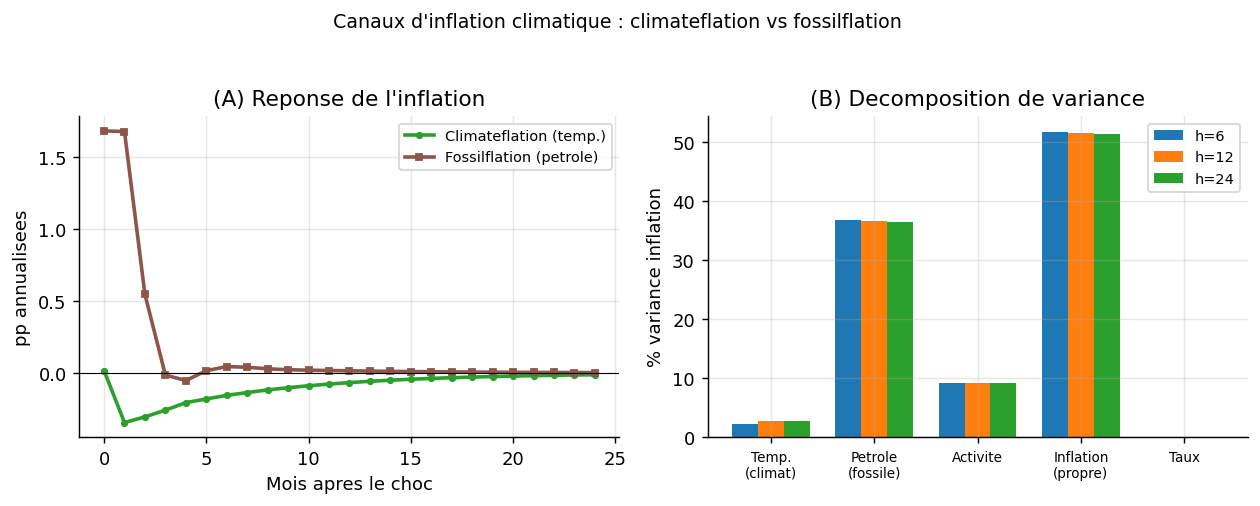
\includegraphics[width=\textwidth]{fig_channels.png}
\end{column}
\end{columns}
\end{frame}

\begin{frame}{Une transmission qui s'intensifie (H3 confirmée)}
\begin{columns}[T]
\begin{column}{0.44\textwidth}
\begin{itemize}\small
\item Local Projections avec interaction « ère récente » ($\geq 2007$).
\item La réponse récente (rouge) domine l'ancienne (bleu).
\item Significatif à \textbf{14--18 mois} : $+1{,}0$ à $+1{,}4$ pp ($t$ jusqu'à $2{,}5$).
\end{itemize}
\vspace{0.4em}
\alert{Ce qui était neutre hier devient inflationniste aujourd'hui.}
\end{column}
\begin{column}{0.56\textwidth}
\centering
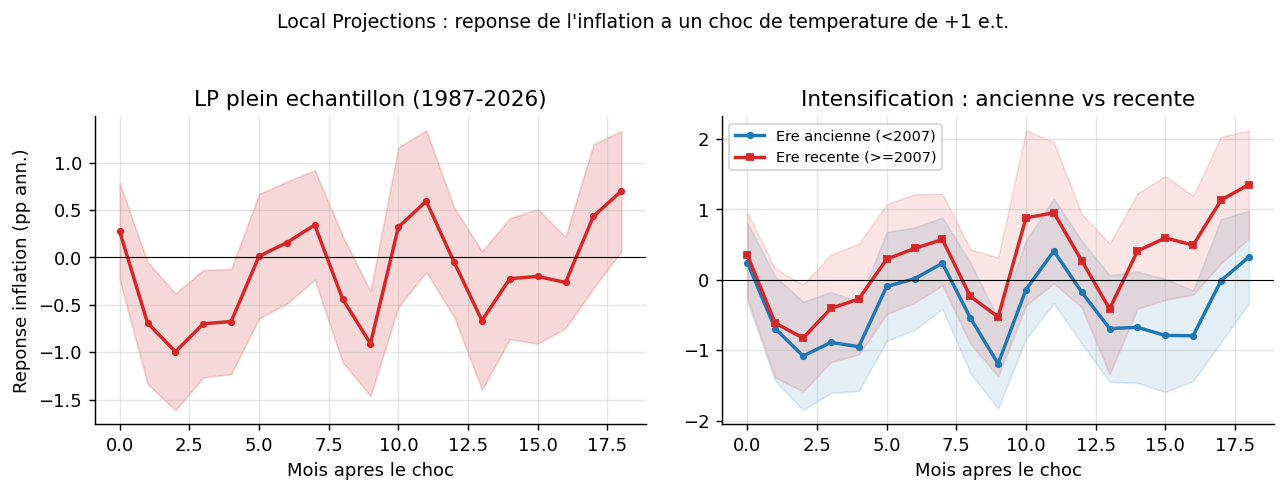
\includegraphics[width=\textwidth]{fig_lp.png}
\end{column}
\end{columns}
\end{frame}

\begin{frame}{Une réponse fortement asymétrique (H4) — le cœur}
\begin{columns}[T]
\begin{column}{0.44\textwidth}
\begin{itemize}\small
\item LP par régime : mois \emph{chaud} vs \emph{froid}.
\item Chocs \alert{chauds} $\to$ inflationnistes ($+2{,}2$ pp cumulés).
\item Chocs \alert{froids} $\to$ désinflationnistes ($-12{,}7$ pp).
\end{itemize}
\vspace{0.4em}
\textbf{Réconciliation :} l'effet \emph{moyen} est faible car chaud et froid se compensent. Mais le réchauffement \emph{multiplie les mois chauds} $\Rightarrow$ effet \emph{net haussier}.
\end{column}
\begin{column}{0.56\textwidth}
\centering

\includegraphics[width=\textwidth]{fig_nonlinear.png}
\end{column}
\end{columns}
\end{frame}

% =====================================================================
% =====================================================================
\begin{frame}[plain]
\begin{center}
{\color{dauphblue}\Large\textbf{Partie 3}}\\[0.4em]
{\large Marchés, robustesse et réponse à la question}
\end{center}
\end{frame}

\begin{frame}{Conséquences pour l'allocation d'actifs}
\begin{columns}[T]
\begin{column}{0.44\textwidth}
\begin{itemize}\small
\item \alert{Obligations} : actif le plus exposé ($\beta=-0{,}26$) — un choc inflationniste érode le nominal.
\item \alert{Or} : couverture ($\beta=+0{,}26$). Actions neutres.
\item Portefeuille \emph{climat-neutre} : on quitte les obligations ($46{,}6\!\to\!36{,}3\%$) pour l'or ($16{,}5\!\to\!38{,}5\%$).
\item Coût : Sharpe $0{,}76\!\to\!0{,}65$ (\alert{$-13{,}6\%$}).
\end{itemize}
\end{column}
\begin{column}{0.56\textwidth}
\centering
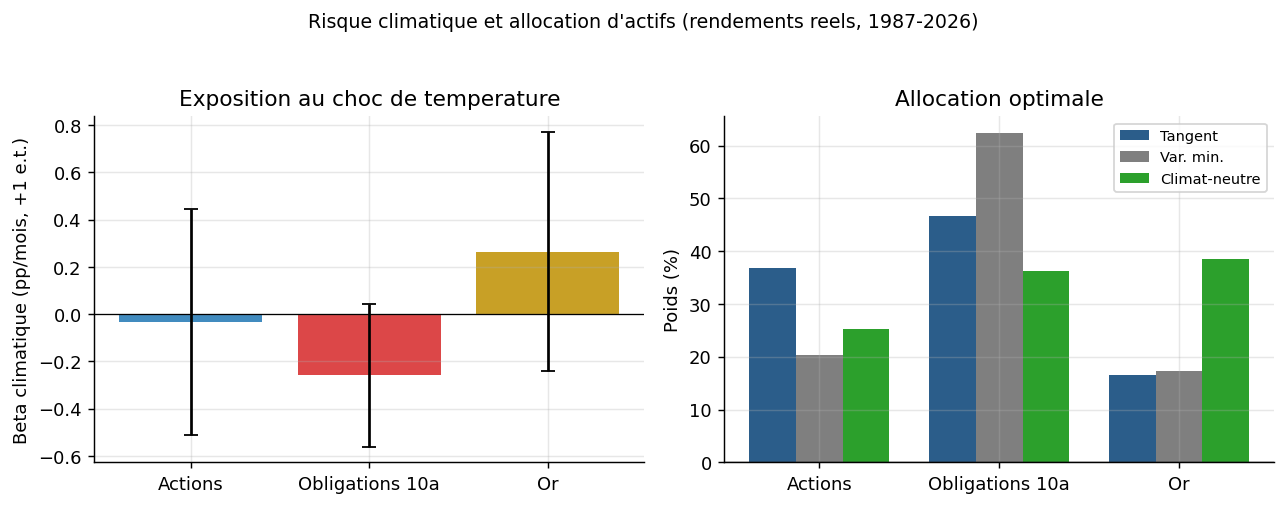
\includegraphics[width=\textwidth]{fig_assets.png}
\end{column}
\end{columns}
\end{frame}

\begin{frame}{Robustesse}
\centering
\small
\begin{tabular}{lcc}
\toprule
Variante & FEVD(24) (\%) & cumul 12 mois (pp) \\
\midrule
Retards $p=2$ (référence) & 2{,}77 & $-2{,}02$ \\
Retards $p=3$ & 3{,}19 & $-2{,}05$ \\
Retards $p=4$ & 3{,}24 & $-2{,}11$ \\
Température ordonnée \emph{en dernier} & 2{,}15 & $-1{,}84$ \\
Détrendage quadratique & 0{,}87 & $-0{,}88$ \\
Détrendage Hodrick--Prescott & 0{,}47 & $-0{,}47$ \\
\bottomrule
\end{tabular}
\vfill
\raggedright\small Part de variance toujours $<\!4\%$ et réponse cumulée toujours négative $\Rightarrow$ \alert{conclusion stable} à l'ordre de Cholesky, au nombre de retards et au détrendage.
\end{frame}

\begin{frame}{La Banque Centrale a-t-elle un rôle ? — réponse nuancée}
\textbf{\color{dauphblue}Non}, pas de cible d'inflation directe :
\begin{itemize}\small
\item effet agrégé trop faible ; réagir mécaniquement amplifierait la perte d'activité (\emph{looking through}).
\end{itemize}
\vspace{0.3em}
\textbf{\color{dauphblue}Mais oui}, un rôle, de trois natures :
\begin{itemize}\small
\item \alert{Prospectif} : intégrer le climat à la fonction de réaction (transmission croissante \& asymétrique vers le haut).
\item \alert{Canal fossile} : accompagner la transition énergétique = stabilité des prix à moyen terme.
\item \alert{Prudentiel} : les obligations (cœur de la transmission \& du bilan) sont l'actif le plus exposé.
\end{itemize}
\vfill
\centering\emph{Le climat ne change pas le mandat ; il change ses conditions d'exercice.}
\end{frame}

\begin{frame}{Conclusion, limites \& extensions}
\textbf{\color{dauphblue}À retenir}
\begin{itemize}\small
\item Effet agrégé faible \& dominé par le fossile, \emph{mais} en intensification, asymétrique, et qui reprice les obligations.
\end{itemize}
\textbf{\color{dauphblue}Limites}
\begin{itemize}\small
\item IPC agrégé (effet concentré sur l'alimentation) ; température globale (proxy) ; activité $\to$ 2015 ; cadre linéaire.
\end{itemize}
\textbf{\color{dauphblue}Extensions}
\begin{itemize}\small
\item Désagréger l'IPC (alimentation/énergie, code fourni) ; panel international ; identification par restrictions de signe.
\end{itemize}
\end{frame}

{\setbeamertemplate{footline}{}
\begin{frame}[plain]
\begin{center}
{\color{dauphblue}\Large\textbf{Merci de votre attention}}\\[0.6em]
{\large Questions ?}\\[1em]
\small Codes \& données reproductibles : \texttt{run\_all.py} (pipeline 01--07).
\end{center}
\end{frame}}

\end{document}